\begin{figure}[!htb]
    \centering
    \begin{subfigure}{\textwidth}
        \centering
        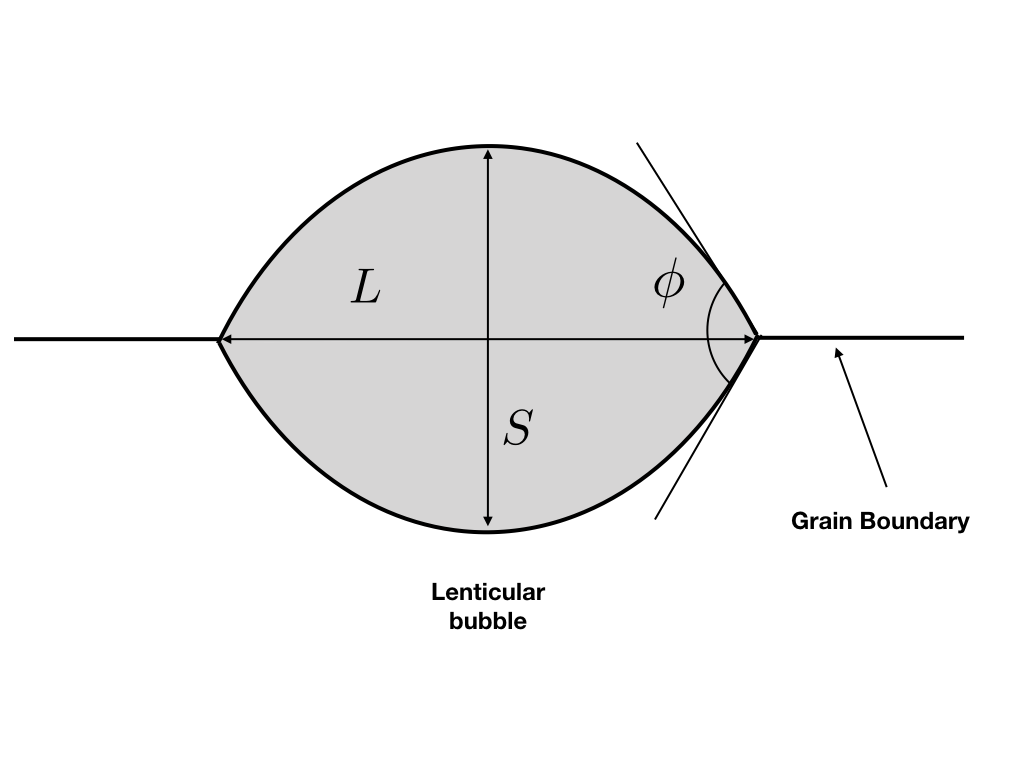
\includegraphics[width=0.6\textwidth]{past/figures/bub.png}
    \end{subfigure}

    \begin{subfigure}{\textwidth}
        \centering
        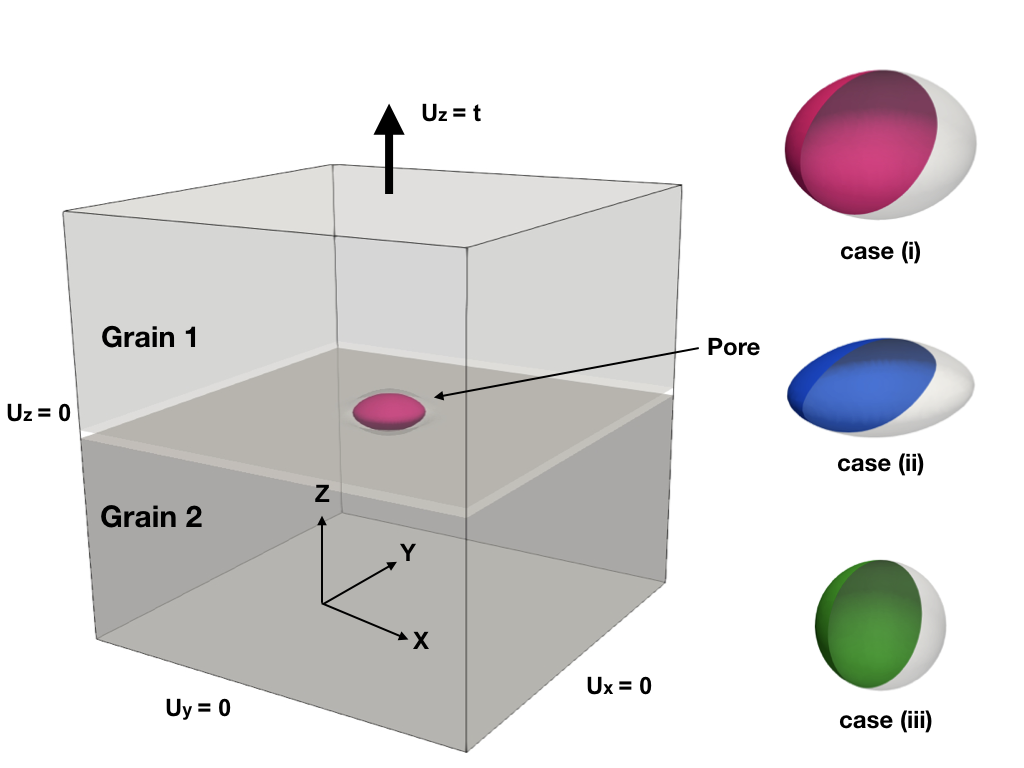
\includegraphics[width=0.6\textwidth]{past/figures/single_ini.png}
    \end{subfigure}

    \vspace{0.1in}
    \begin{tikzpicture}
        \begin{axis}[
            width=\textwidth,
            height=0.6\textwidth,
            ticks=none,
            xlabel=Strain,ylabel=Stress,
            xmin=0,
            xmax=0.006,
            ymin=0,
            ymax=700,
            every axis plot/.append style={line width=1pt}
        ]
            \addplot +[mark=none,color=red!60!black] table[x expr=\thisrowno{2}/40,y=ave_stress_top] {past/data/single_case1.csv};
            \addplot +[mark=none,color=blue!60!black] table[x expr=\thisrowno{2}/40,y=ave_stress_top] {past/data/single_case2.csv};
            \addplot +[mark=none,color=green!60!black] table[x expr=\thisrowno{2}/40,y=ave_stress_top] {past/data/single_case3.csv};
        \end{axis}
    \end{tikzpicture}
\end{figure}
